\documentclass[11pt]{article}
\usepackage{graphicx}
\usepackage{amsmath}
\usepackage{float}


    \title{\textbf{Project-1}}
    \author{\textbf{Ameya Konkar} \; \textbf{UID: 118191058}}
    
    \addtolength{\topmargin}{-3cm}
    \addtolength{\textheight}{3cm}
    
\begin{document}

\maketitle
\thispagestyle{empty}

\section{AR tag Detection }
As per the task, AR tag detection using Fast Fourier Transform was performed on a selected frame of the video. The purpose of this task is to filter the image. Instead of convoluting the image using a kernel, converted the image in Frequency domain using Fourier transform. Hence, any filter can directly be multiplied on the image instead of iterating through the image. The steps followed are as follows:\\
\begin{description}

\addtolength{\itemindent}{0.80cm}
\itemsep0em 
\item[1.] Converted the image to gray scale.
\item[2.] Threshold the image.
\item[3.] Used Fast Fourier transform on the image.
\item[4.] Created a circular mask and added to the image.
\item[5.] Used Inverse Fast Fourier Transform to filter the image.

\begin{figure}[!htbp]
  \centering
	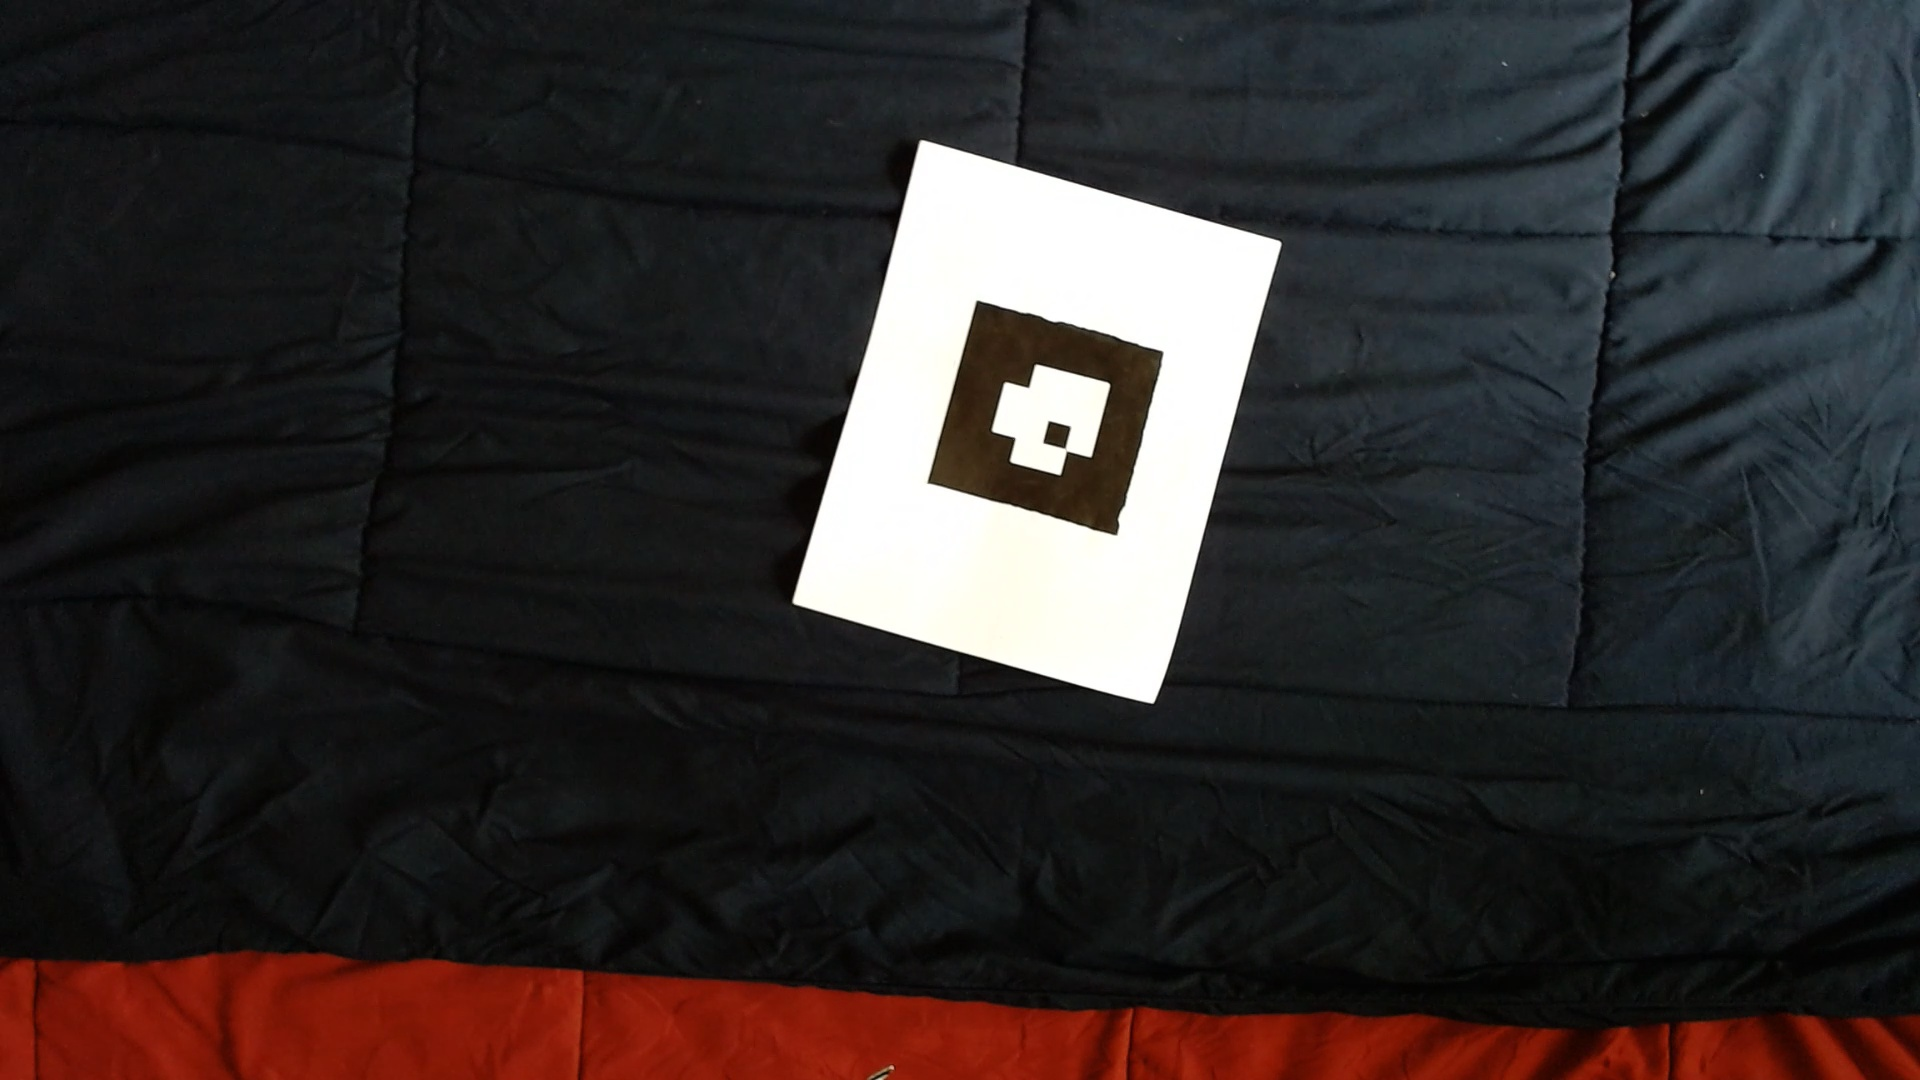
\includegraphics[width=1\textwidth]{frame15}
	\caption{Original Image.}
	\
\end{figure}

\begin{figure}[!htbp]
  \centering
	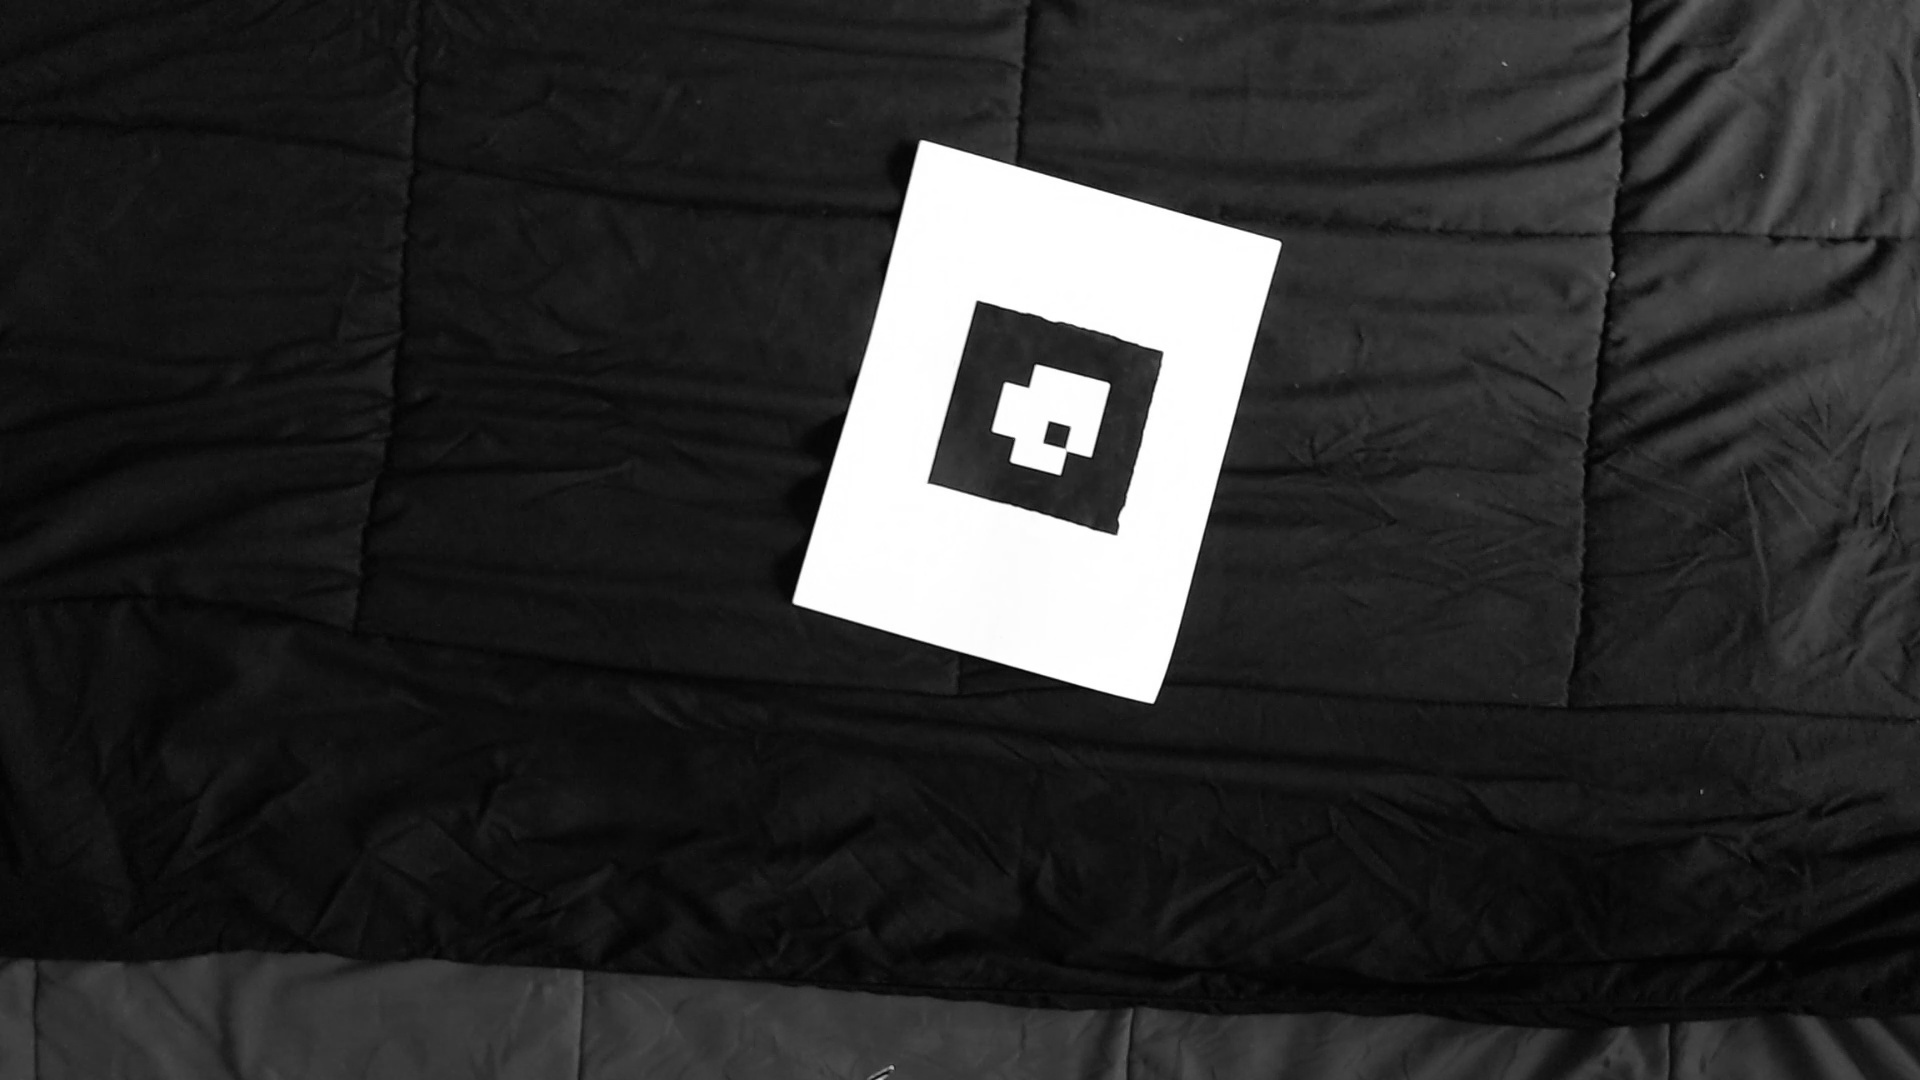
\includegraphics[width=1\textwidth]{Grayscale}
	\caption{Grayscale Image.} 
\end{figure}

\begin{figure}[!htbp]
  \centering
	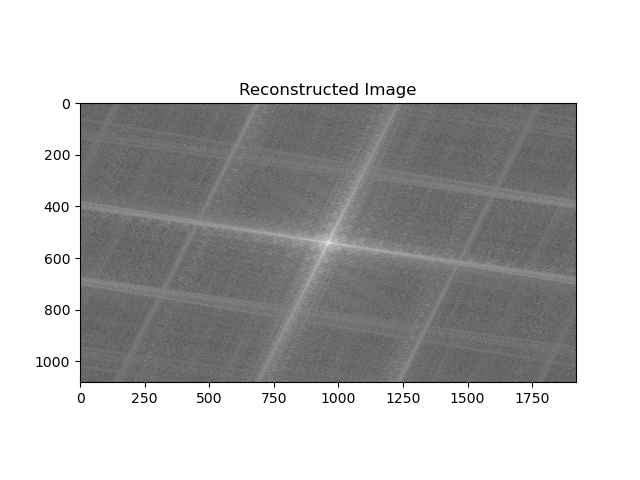
\includegraphics[width=1\textwidth]{FFT}
	\caption{FFT Image.} 
\end{figure}
\begin{figure}[!htbp]
  \centering
	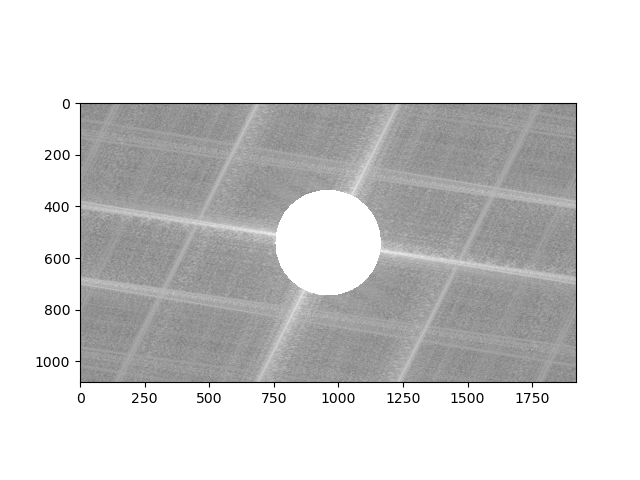
\includegraphics[width=1\textwidth]{FFTmasked}
	\caption{FFT with mask Image.} 
\end{figure}
\begin{figure}[!htbp]
  \centering
	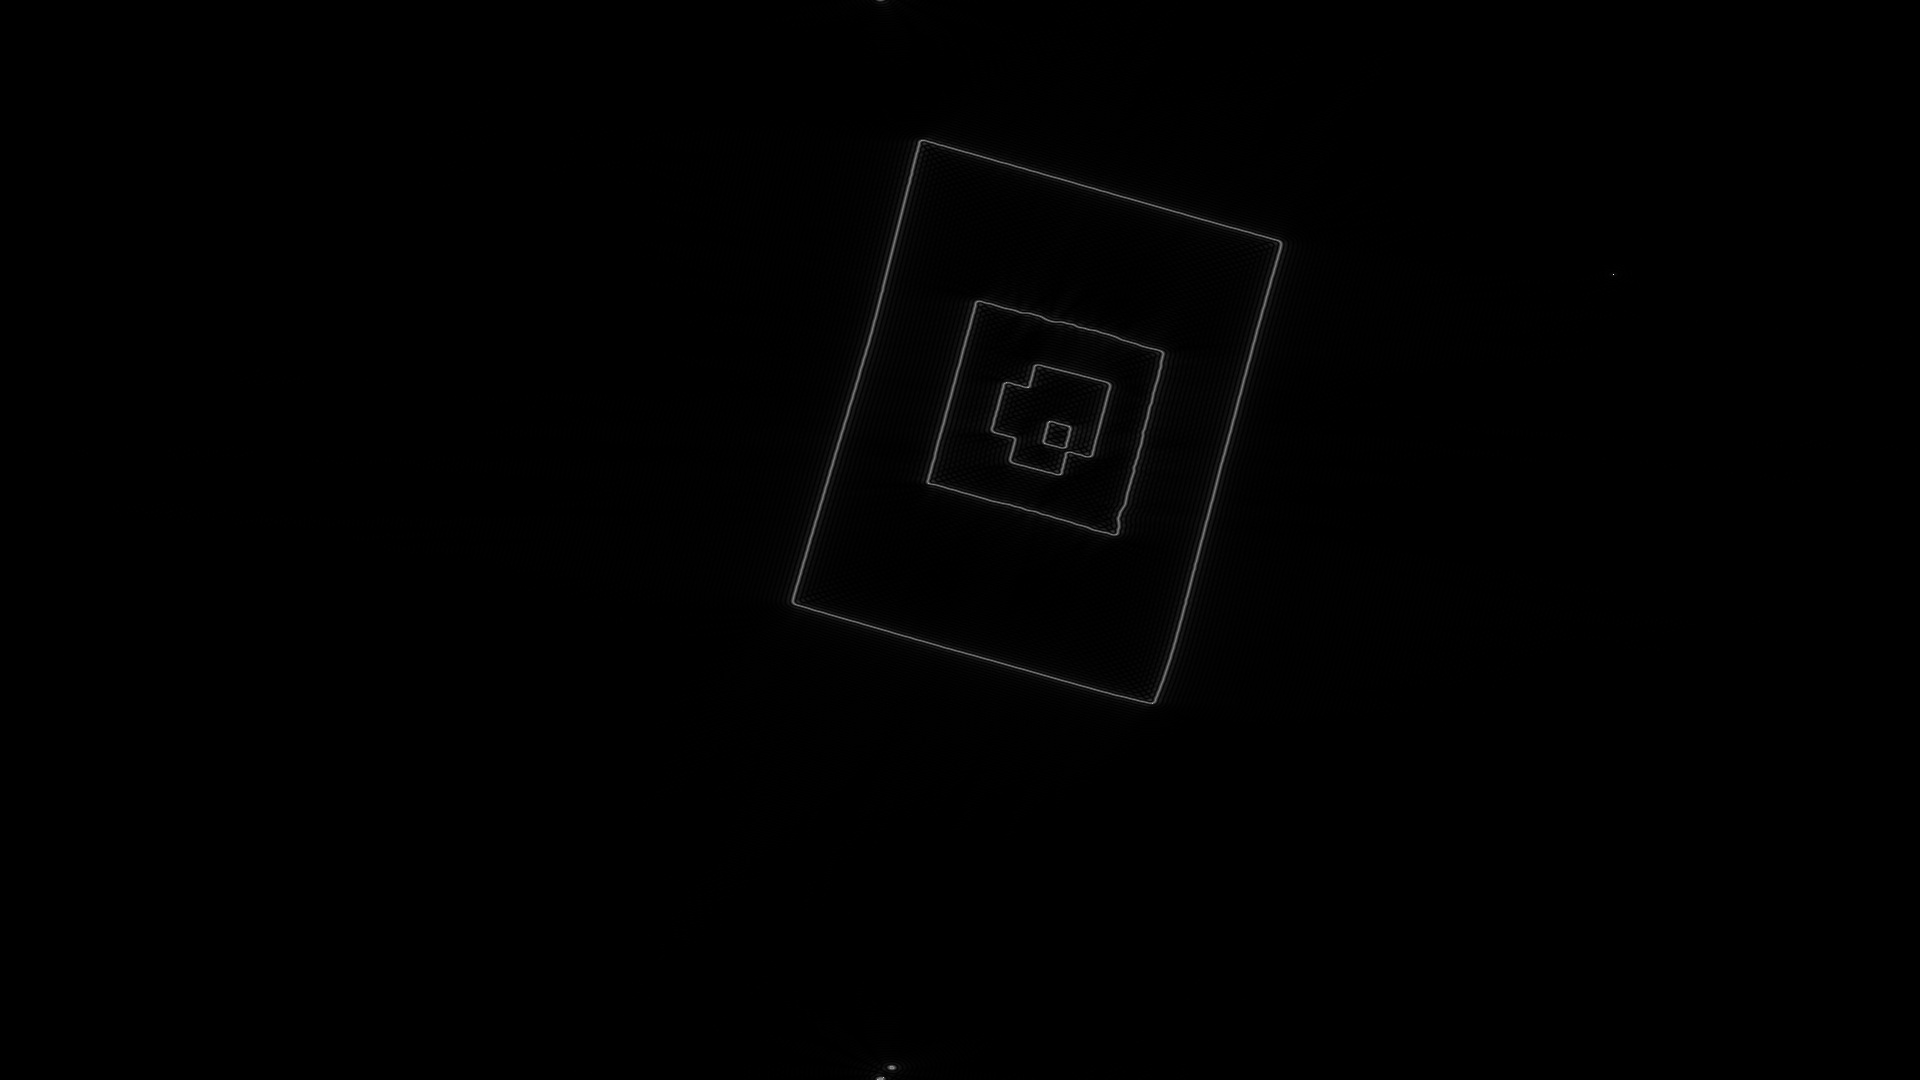
\includegraphics[width=1\textwidth]{FFTimage}
	\caption{Filtered Image.} 
\end{figure}
\end{description}

\section{Decode custom AR tag}
As per the given task, Id of the AR tag of a selected frame of the video was performed. The following steps were used to detect the AR tag:
\begin{description}

\addtolength{\itemindent}{0.80cm}
\itemsep0em 
\item[1.] Convert the image to grayscale.
\item[2.] Threshold the image.
\item[3.] Use cv.Floodfill to remove background(black) pixels outside the page containing the AR tag.
\item[4.] Detected Corners using cv2.goodFeaturesToTrack and selected four extreme corners representing the corners of the AR Tag.
\item[5.] Assumed four world coordinates as \textbf{[\ minx, miny]\ ,[\textbf {maxx, miny}]\ ,[\ minx, maxy]\, [\ maxx, maxy]}\ out of the corner of the AR tag.
\item[6.] Did compute the Homography matrix \textbf{H} =
			$\begin{bmatrix}
			h_{00} & h_{01} & h_{02}\\
			h_{10} & h_{11} & h_{12}\\
			h_{20} & h_{21} & h_{22}
			\end{bmatrix}$ using \textbf{A} matrix. The Homography matrix is eigen vector corresponding to the least eigen value.
\item[7.] Computed homography matrix multiplication on every pixel from the AR tag to get new coordinates in the world space. Filled colors of the respective image space pixel to a world space pizel. 
\item[8.] After finding the isolated AR tag, divided the image into 8 parts. Checked the value of the pixels corresponding to the coordinates [\ 3.5d, 3.5d]\ ,[\ 4.5d, 3.5d]\ ,[\ 4.5d, 4.5d]\, [\ 3.5d, 4.5d]\ in clockwise order. If the value is 255, cosidered it as 1 else 0. 
\item[9.] If a value of 7 is found by using bit operation counter-clockwise, then the orientation is correct, otherwise rotate the AR Tag till the bit operation of 13 is found.
\end{description}

\begin{figure}[!htbp]
  \centering
	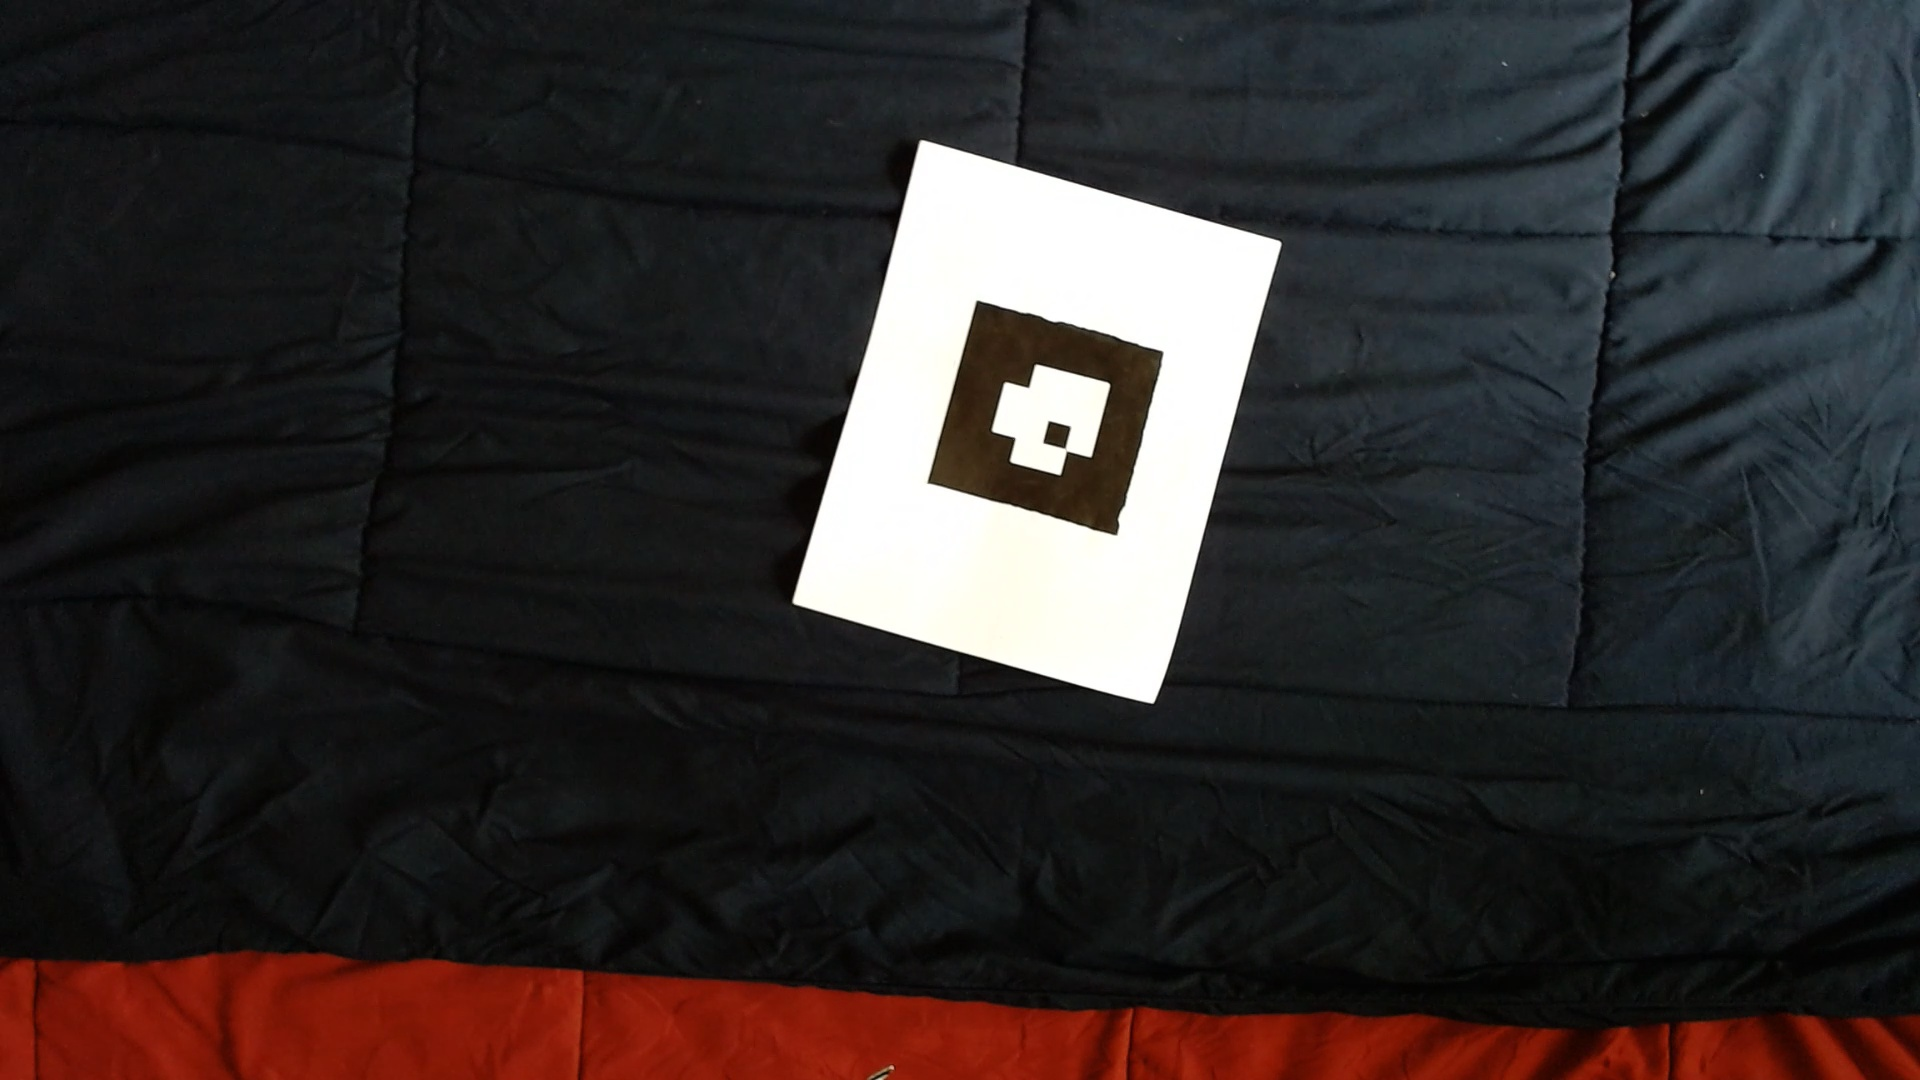
\includegraphics[width=1\textwidth]{frame15}
	\caption{Original Image.}
\end{figure}

\begin{figure}[!htbp]
  \centering
	
\includegraphics[width=1\textwidth]{ThresholdedImage}
	\caption{Thresholded Image}
\end{figure}
\begin{figure}[!htbp]
  \centering
	
\includegraphics[width=1\textwidth]{floodfill}
	\caption{Flood fill algorithm to isolate the AR tag.}
\end{figure}

\begin{figure}[!htbp]
  \centering
	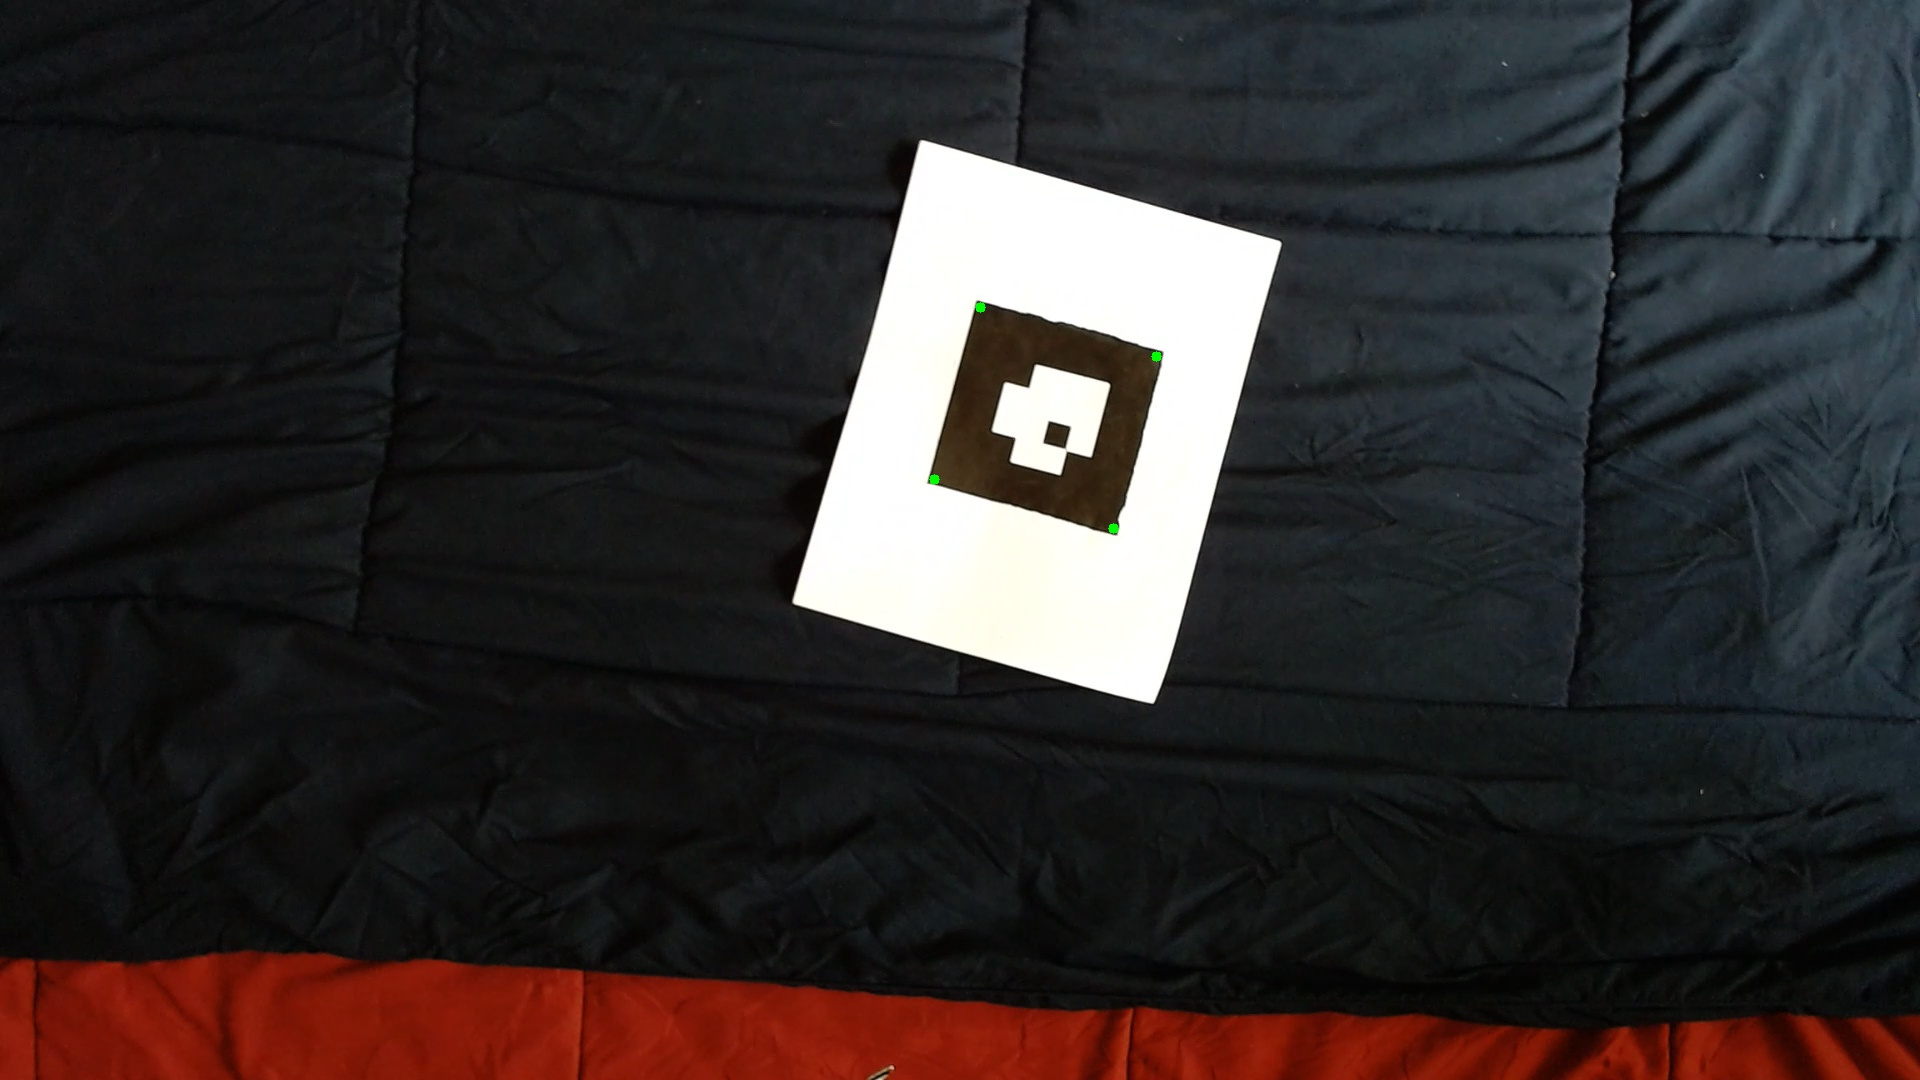
\includegraphics[width=1\textwidth]{cornersARTag}
	\caption{Corners Detected.}
\end{figure}

\begin{figure}[!htbp]
  \centering
	
\includegraphics[width=0.5\textwidth]{AR_Code_Homography}
	\caption{AR Tag detected.}
\end{figure}

\section{Superimposing image onto Tag}
After detecting the AR Tag value, The following steps were followed to superimpose the Terp image onto the AR tag.
\begin{description}
\addtolength{\itemindent}{0.80cm}
\itemsep0em 
\item[1.] Rotate the terp image based on the number of rotations required to detect the AR tag.
\item[2.] Resized the terpImage to the AR tag image.
\item[3.] Used inverse homography to find image coordinates corresponding to world coordinates and filled the pixels with color of the terpImage pixels
\item[4.] Used the above process on all the frames of the video.
\end{description}

\begin{figure}[!htbp]
  \centering
	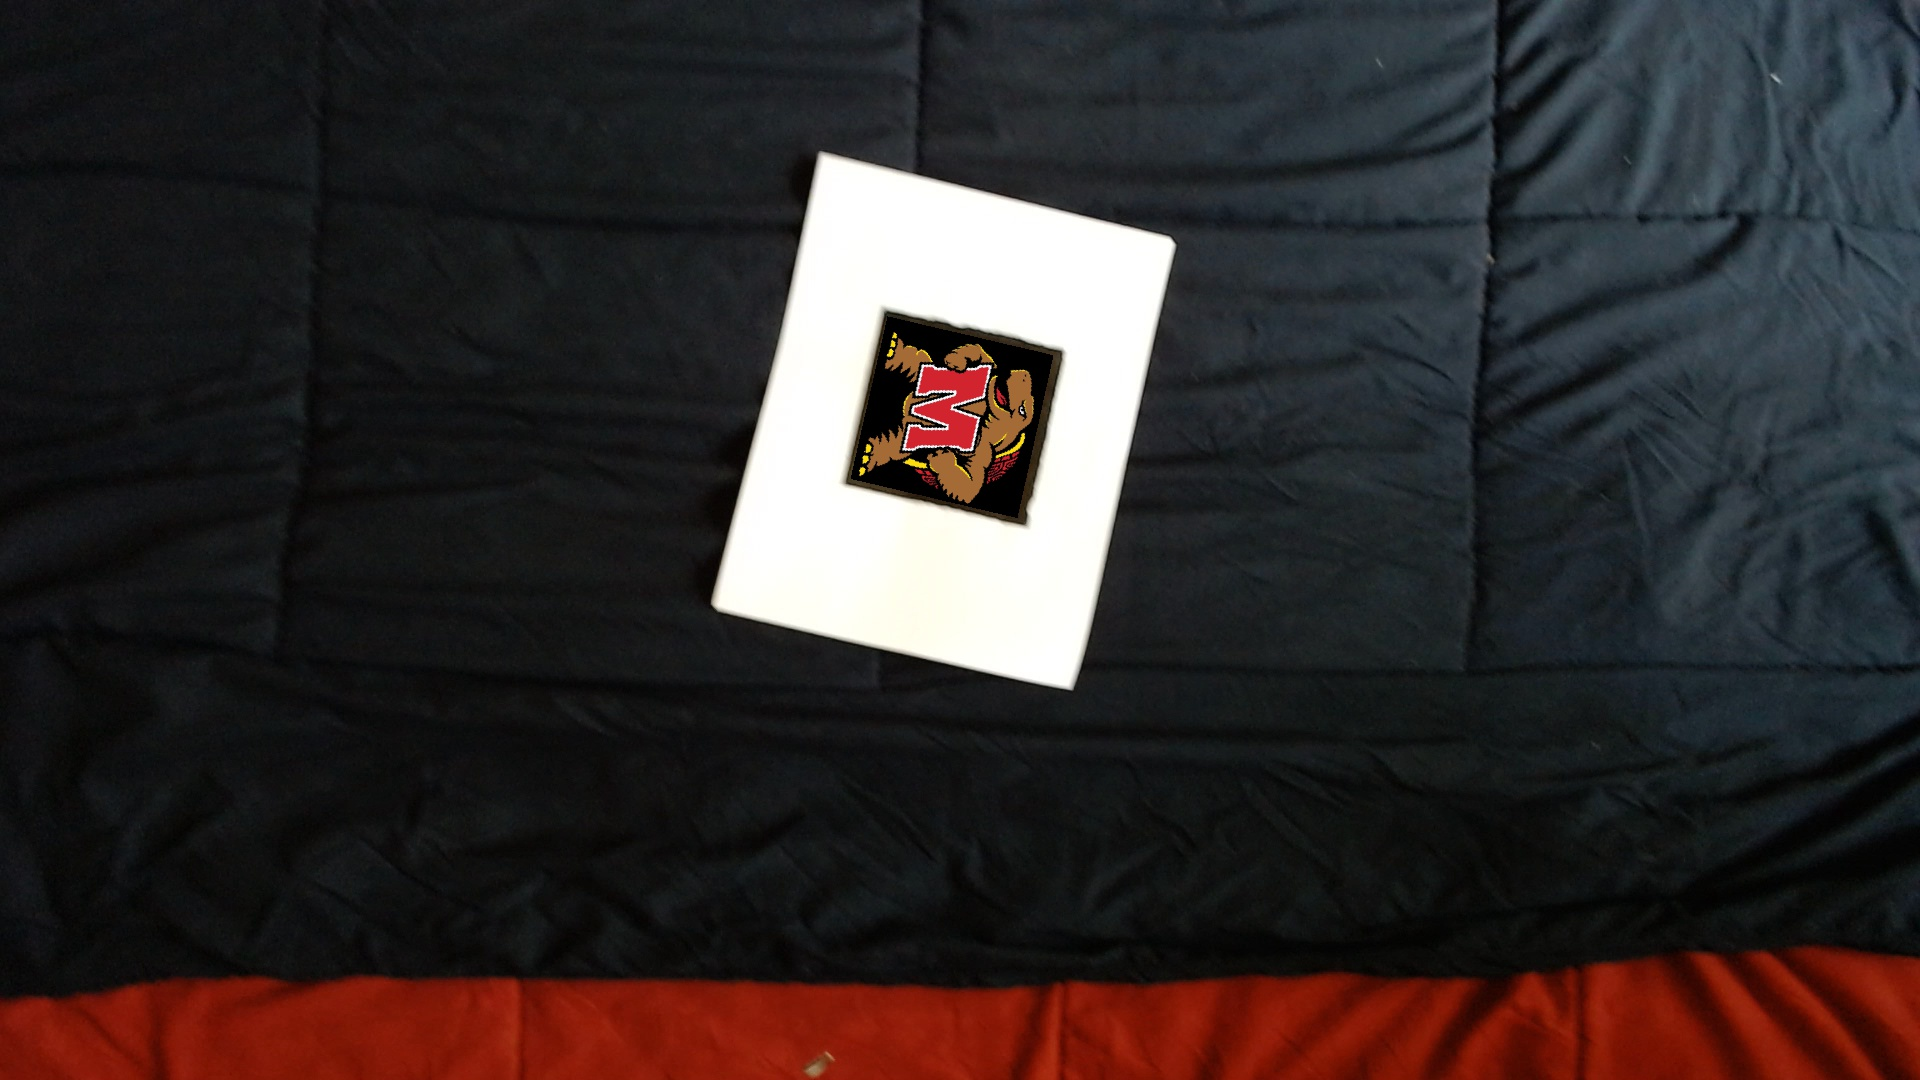
\includegraphics[width=1\textwidth]{terpSuperimposed}
	\caption{Superimposed Terp image.}
\end{figure}

\section{Placing a virtual cube onto Tag}
After detecting the AR Tag value, The following steps were followed to place the virtual cube on the tag.
\begin{description}
\addtolength{\itemindent}{0.80cm}
\itemsep0em 
\item[1.] Used the intrensic matrix \textbf{K} = 
			$\begin{bmatrix}
			1346.100595 & 0 & 932.1633975 \\
			0 & 1355.933136 & 654.8986796\\
			0 & 0 & 1
			\end{bmatrix}$.
 and Homography matrix \textbf{H} to compute the matrix \textbf{P} = 
			$\begin{bmatrix}
			r1_{00} & r2_{01} & r3_{02} & t_{02}\\
			r1_{10} & r2_{11} & r3_{12} & t_{12}\\
			r1_{20} & r2_{21} & r3_{22} & t_{22}
			\end{bmatrix}$.
			such that \[\textbf{B} = lambda*K^{-1}*H\] and 
			\[\textbf{lambda} = [(||K^{-1}*h1|| + ||K^{-1}*h2||)/2]^{-1}\]
			Here,  \[\textbf{B} = \begin{bmatrix} 
									b1 & b2 & b3
									\end{bmatrix}. \] and 
									\[\textbf{r1} = lambda*b1,\; \textbf{r2} 										= lambda*b2,\; \textbf{r3} = r1\times r2,\; \textbf{r3} = lambda*b3\] 
\item[2.] Multiplied the P matrix with the four world coordinates (\ height is taken to be -200 )\
\item[3.] Created a cube out of the corners of the AR tag and the new coordinates found.
\item[4.] Used the above process on all the frames of the video.
\begin{figure}[!htbp]
  \centering
	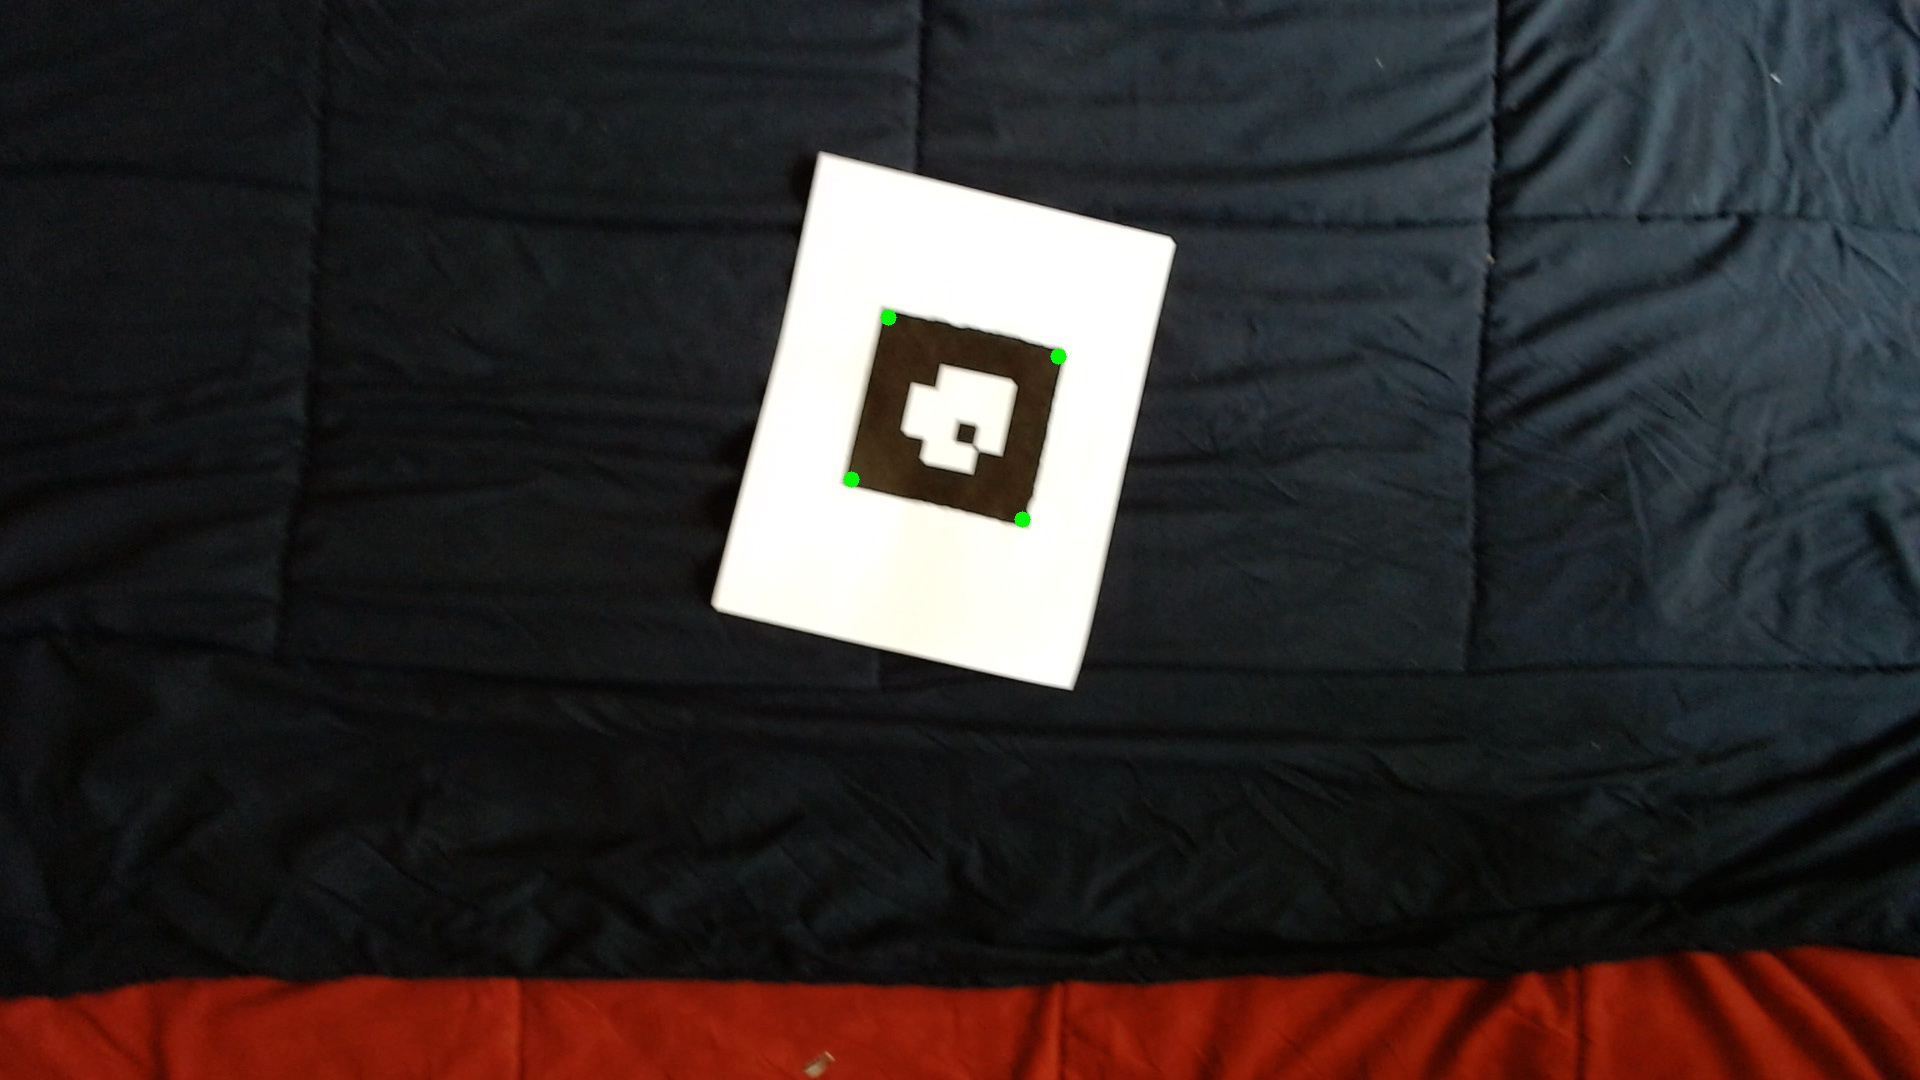
\includegraphics[width=1\textwidth]{Corners}
	\caption{Corners detected.}
\end{figure}

\begin{figure}[!htbp]
  \centering
	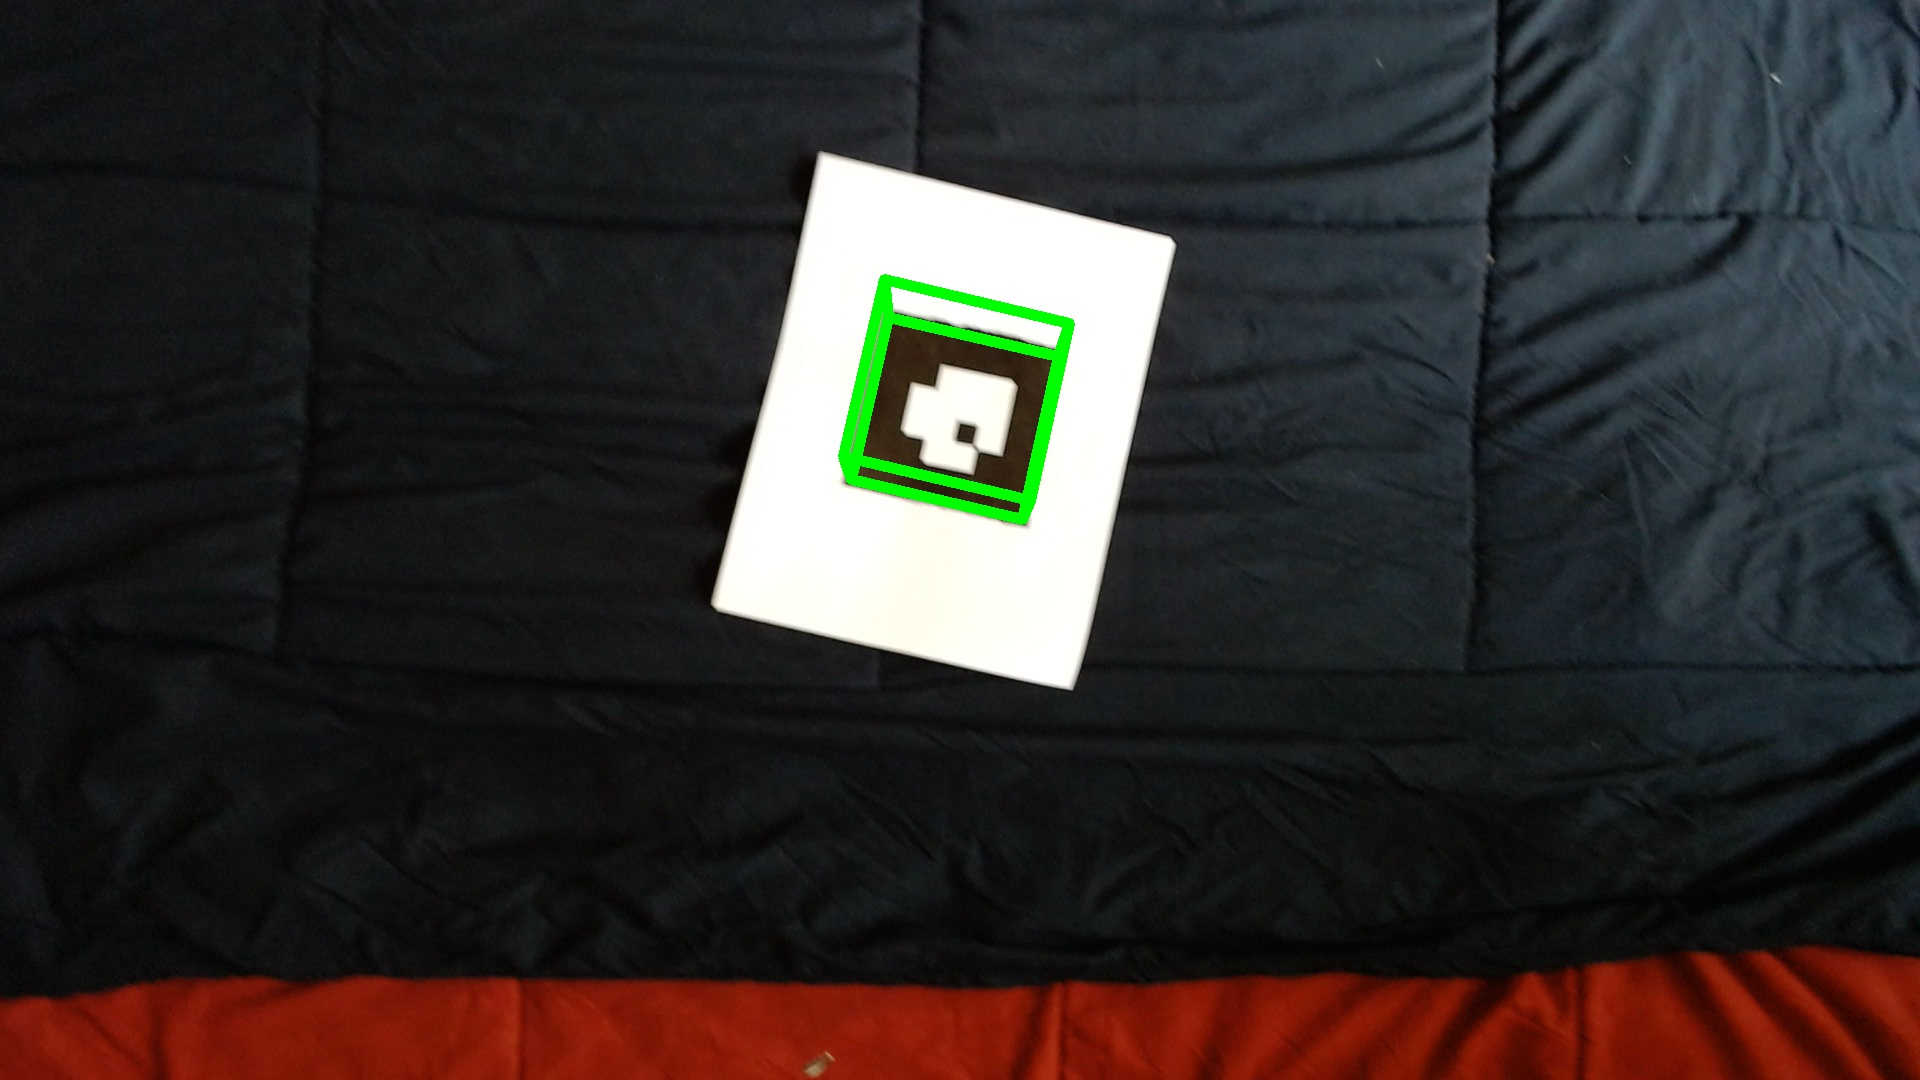
\includegraphics[width=1\textwidth]{Cube}
	\caption{Cube superimposed on the AR tag.}
\end{figure}
\end{description}

\end{document}

